%%%%%%%%%%%%%%%%%%%%%%%%%%%%%%%%%%%%%%%%%
% Simple Sectioned Essay Template
% LaTeX Template
%
% This template has been downloaded from:
% http://www.latextemplates.com
%
% Note:
% The \lipsum[#] commands throughout this template generate dummy text
% to fill the template out. These commands should all be removed when 
% writing essay content.
%
%%%%%%%%%%%%%%%%%%%%%%%%%%%%%%%%%%%%%%%%%

%----------------------------------------------------------------------------------------
%	PACKAGES AND OTHER DOCUMENT CONFIGURATIONS
%----------------------------------------------------------------------------------------

\documentclass[12pt]{article} % Default font size is 12pt, it can be changed here

\usepackage{amsmath}

\usepackage{geometry} % Required to change the page size to A4
\geometry{a4paper} % Set the page size to be A4 as opposed to the default US Letter

\usepackage{graphicx} % Required for including pictures

\usepackage{float} % Allows putting an [H] in \begin{figure} to specify the exact location of the figure
\usepackage{wrapfig} % Allows in-line images such as the example fish picture

\usepackage{lipsum} % Used for inserting dummy 'Lorem ipsum' text into the template

\linespread{1.2} % Line spacing

%\setlength\parindent{0pt} % Uncomment to remove all indentation from paragraphs

\graphicspath{{Pictures/}} % Specifies the directory where pictures are stored

\begin{document}

%----------------------------------------------------------------------------------------
%	TITLE PAGE
%----------------------------------------------------------------------------------------

\begin{titlepage}

\newcommand{\HRule}{\rule{\linewidth}{0.5mm}} % Defines a new command for the horizontal lines, change thickness here

\center % Center everything on the page

\textsc{\LARGE University of Houston Clear Lake}\\[1.5cm] % Name of your university/college
\textsc{\Large CSCI 4362}\\[0.5cm] % Major heading such as course name
\textsc{\large Game Programming}\\[0.5cm] % Minor heading such as course title

\HRule \\[0.4cm]
{ \huge \bfseries Proposal: Balls To The Wall}\\[0.4cm] % Title of your document
{ \bfseries Level Up Solutions}\\[0.2cm] % Title of your document
\HRule \\[1.5cm]

\begin{minipage}{0.4\textwidth}
\begin{flushleft} \large
\emph{Authors:}\\
Mike Moore, \newline
Tom, \newline
Mike} % Your name
\end{flushleft}
\end{minipage}
~
\begin{minipage}{0.4\textwidth}
\begin{flushright} \large
\emph{Professor:} \\
Dr. Pradeep Buddharaju % Supervisor's Name
\end{flushright}
\end{minipage}\\[4cm]

{\large \today}\\[3cm] % Date, change the \today to a set date if you want to be precise

%
\includegraphics{UHCLLogo}\\[0.5cm] % Include a department/university logo - this will require the graphicx package

\vfill % Fill the rest of the page with whitespace

\end{titlepage}

%----------------------------------------------------------------------------------------
%	TABLE OF CONTENTS
%----------------------------------------------------------------------------------------

\tableofcontents % Include a table of contents

\newpage % Begins the essay on a new page instead of on the same page as the table of contents 

%----------------------------------------------------------------------------------------
%	Game Overview
%----------------------------------------------------------------------------------------

\section{Game Overview} % Major section
Balls to the Wall (BtW) is a 2d puzzle game. It requires a combination of strategy and precision. The game supports both a single
and multiplayer mode. The object of the game is to direct as many bouncing balls into the player's basket as possible.
The player has a set of blocks, and they must use these blocks to direct a bouncing ball on a trajectory that will
land the ball in the player's immovable basket. Points are rewarded for each ball that makes it into the basket, and they are deducted
for misses. Points are also rewarded once per ball/block collision. A skillfull player will direct the ball on a long
trajectory in which the ball bounces off several blocks before landing in the basket. This is called chaining collisions,
and is a quick way towards a high score. A diagram of the gameplay is shown in figure 1.

\begin{figure}[H] % Gameplay image
\center{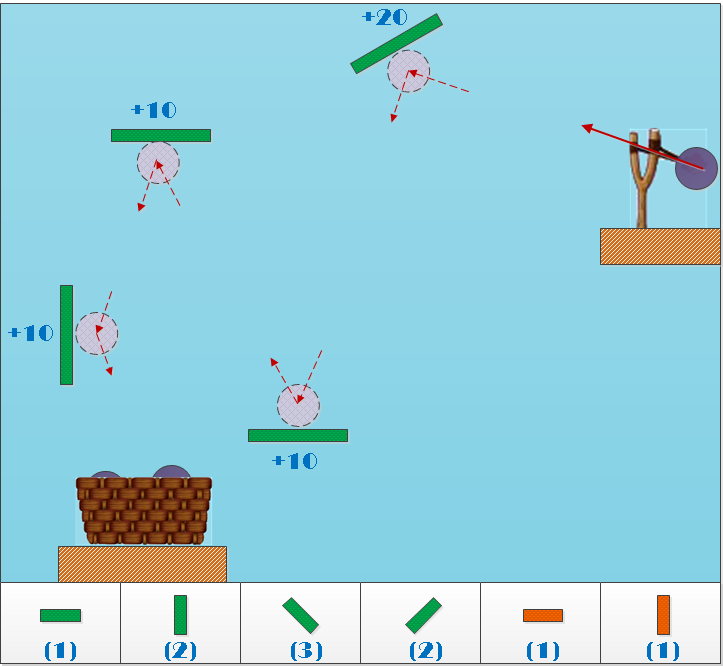
\includegraphics[width=0.75\linewidth]{GMockUp}}
\caption{BtW Gameplay.}
\label{fig:speciation}
\end{figure}

At the beginning of each level the player is given a set of blocks. Blocks come in several different types. The player can use any combination of
simple horizontal blocks, angled blocks, and vertical blocks. All blocks have a pre-defined material strength property. Wood blocks are weaker than
concrete blocks, and steel blocks are the strongest.

%----------------------------------------------------------------------------------------
% Single Player Mode Section
%----------------------------------------------------------------------------------------
\section{Single Player Mode} % Major section

The single player version of the game focuses on the player progressing through a series of increasingly difficult levels.
Once a level starts, bouncing balls are shot out of a slingshot and they begin falling within the level. The initial velocity
for each ball will be random over a restricted angular range. The player's job is to quickly place his blocks in order to direct each
ball into the basket. The ball will collide with blocks and bounce off of them according to the physics of semi-elastic collisions. 
The player loses points if the ball misses the cup or flys out of view. The player gains points for each ball made into the cup, and for each ball/block 
collision that they are able to chain together.

It's important to remember that a player's blocks must be placed. A player is not allowed to have one block follow their game cursor around. 
The player must place and release their block prior to any ball/block collision. This forces the player to carefully time their block placement. Success
in this game will require strategic management of a player's blocks, and block placement precision.

%----------------------------------------------------------------------------------------
% Two Player Mode Section
%----------------------------------------------------------------------------------------
\section{Two Player Mode} % Major section
BtW can also be played in two player mode. Both networked, and shared screen mode will be supported. Multiplayer gameplay closely matches
the single player mode with a few key differences. In two player mode, players will take turns either placing blocks and directing incoming 
balls towards their basket, or they will wreak havoc by carefully slingshotting balls in the worst possible direction for
their oponent. The two players will take turns progressing through a set of levels. Each are competing to score higher than the other.

More detail is needed here.... New screenshot could help.

%------------------------------------------------

%\subsection{Subsection 1} % Sub-section

%\lipsum[1] % Dummy text

%------------------------------------------------

%----------------------------------------------------------------------------------------
%	Game Physics Section 
%----------------------------------------------------------------------------------------

\section{Game Physics} % Major section
BtW relies heavily on a mathematical model for `semi-elastic' collisions in the two dimensional
game space. This section is dedicated to describing this mathematical model and deriving the equations
of motion for the bouncing balls.

The collisions between a bouncing ball and a block are modelled as `semi-elastic'. This means
that energy is removed from the ball after a collision with a block. The intent is to add an
an element of strategy to the game. A player's block is capable of slowing
down the ball's velocity after each collision. This makes the ball's trajectory more manageable
for the player, but it comes at the expense of the block's `health'. Blocks can only sustain a certain
number of collisions before they crumble and dissapear from the game environment. In the next
sections, we will derive the equations of motion for the bouncing ball.

%------------------------------------------------

\subsection{ Reference Frame Definition} % Sub-section
Before deriving the equations of motion, it will be important to define our reference frames.
BtW has only two types of reference frames. The first reference frame is the Game Frame (G.F.).
This is the inertial reference frame in which all game components translate through the game's
two dimensional environment. The origin will be taken to be at the bottom left corner of the 
visible game-play space. The second type of reference frame is the Block Frame (B.F.). This system
is primarily defined by the block's surface normal, and has its origin at the top-center portion
of the block. A diagram of both frames is included below.

\begin{figure}[H] % Reference Frame image
\center{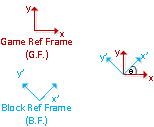
\includegraphics[width=0.25\linewidth]{RefFrames}}
\caption{BtW Reference Frames.}
\label{fig:speciation}
\end{figure}

With these reference frames defined, we can next define the simple transformation equations
from the G.F. to the B.F. This transformation will be important, as we will derive the collision
equations in the B.F. and then rely on the transformation matrix to convert back into the G.F. That way we
can update the G.F. velocity vector of the ball after the collision mathematics are calculated in the B.F.

The transformation is defined as follows:

\[
\left[\vec{v_{b}}\right]^{G.F.} =
  \begin{bmatrix}
    \cos{\theta} & -\sin{\theta}\\
    \sin{\theta} & \cos{\theta}\\
  \end{bmatrix}
  \left[\vec{v_{b}}\right]^{B.F.}
\]

%\begin{wrapfigure}{l}{0.4\textwidth} % Inline image example
%  \begin{center}
%    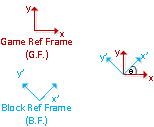
\includegraphics[width=0.5\textwidth]{RefFrames}
%  \end{center}
%  \caption{BtW Reference Frames}
%\end{wrapfigure}

\subsubsection{Kinematics} % Sub-sub-section

The equations describing the two dimensional motion of the bouncing balls come from elementary
kinematics. A drag coefficient is added in order to model the drag force acting on each ball
as it moves through the air. If this were not done, the ball would only lose energy during
each semi-elastic collision and not during its flight through the `air'. The equations used for
each bouncing ball are listed below. All vectors are in the G.F.

\[
\vec{a_{b}} =
  \begin{bmatrix}
    0 \\
    -g \\
  \end{bmatrix}
\]

\[ \vec{v}_{b} = \vec{v}_{b0} -C_{d}\vec{v}_{b}^{\hspace{1mm}\prime}+\vec{a_{b}}\Delta t \]

\[ \vec{p}_{b} = \vec{p}_{b0}  + \vec{v}_{b} \Delta t + \frac{\vec{a_{b}}\Delta t^{2}}{2} \]

Where $\vec{a_{b}}$ is the ball's acceleration in the G.F, $\vec{v}_{b}$ is the ball's velocity in 
the G.F., and $\vec{p}_{b}$ is the ball's position in the G.F. The rest of the terms are constants.
$\Delta t$, $C_{d}$, $\vec{v}_{b0}$, $\vec{p}_{b0}$ represent the time step, drag coefficient, initial
velocity (G.F.), and initial position (G.F.), respectively.


%------------------------------------------------

\subsubsection{Semi-Elastic Collisions} % Sub-sub-section

With the relevant reference frames and ball kinemtics defined, we can turn to 
the physics of ball/block collisions. For mathematical and notational convenience,
we will derive the collision equations in the block's reference frame (B.F.). We will
assume that the colliding ball's angle of incidence, $\alpha$, equals the ball's angle of
reflection. Furthermore, we will add a coefficient of damping into the collision equations
which will come to represent the energy loss that the bouncing ball experiences due to the collision
with the block. This damping coefficient is held constant during a given collision, but it will 
vary in proportion to the inverse of the block's strength on each subsequent collision.
A block will always lose some strength following each ball/block collision. As the block loses strength, the
collision equations will remove more and more energy from the reflecting ball. This will occur until
the block's strength reduces below a threshold. At that point, the block will dissapear, and collisions
will no longer occur at that particular block.

The figure below depicts an arbitrary ball/block collision. The angle's have been parameterized in 
order to derive equations that will apply to all possible ball/block collisions in BtW.

\begin{figure}[H] % Reference Frame image
\center{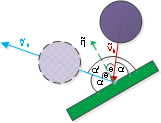
\includegraphics[width=0.45\linewidth]{GPhysicsModel}}
\caption{BtW Collision Diagram.}
\label{fig:speciation}
\end{figure}


In this diagram, $\vec{n}$ is the vector normal to the block's surface. This vector defines the block's reference
frame (B.F.). In all cases, the block frame x-axis will be defined $90^{\circ}$ clockwise from $\vec{n}$. The
B.F. y-axis will aways point in the direction of $\vec{n}$. All block rotations will occur about the B.F. z-axis,
which will be defined as a vector pointing out of the page and perpendicular to the x and y axes.

Define $\vec{v_{b}}$ as the incoming ball's velocity vector expressed in the B.F. Likewise, define $\vec{v_{b}}^{\prime}$
as the reflecting ball's velocity vector also expressed in the B.F. We would like to calculate the reflecting ball's
velocity vector immediately following the semi-elastic collision with block. To do that, let's define $\alpha $ as the
collision incidence and reflection angle. The geometry of the figure defines the remaining angles. Let
$d_{\epsilon}$ represent the amount of energy removed from the reflecting ball following the collision. The collision 
equations become:


\[ \theta  = \pi - cos^{-1}\left(\frac{\vec{v_{b}}\cdot\vec{n}}{\left|\vec{v_{b}}\right|\left|\vec{n}\right|}\right) \]
\[\alpha = \frac{\pi}{2}  - \theta \]
\[ \alpha^{\prime} = \alpha + 2\theta \]
\[
\vec{v_{b}}^{\prime}\right =
  d_{\epsilon}\left|\vec{v_{b}}\right|
  \begin{bmatrix}
    \cos\alpha^{\prime}\\
    \sin\alpha^{\prime}\\
  \end{bmatrix}

\]

They key equation is the one calculating the reflecting ball's velocity vector given the geometry of the collision and
the damping factor, $d_{\epsilon}$.

%----------------------------------------------------------------------------------------
%	Software Architecture Section
%----------------------------------------------------------------------------------------
\section{Software Architecture} % Major section

Section TODO.

Fill out section with software architecture diagram. Describe system, subsystems, and
classes within each subsystem.

%\section{Content Section}

%\subsection{Subsection 1} % Sub-section

% Content

%------------------------------------------------

%\subsection{Subsection 2} % Sub-section

% Content

%----------------------------------------------------------------------------------------
%	CONCLUSION
%----------------------------------------------------------------------------------------

%\section{Conclusion} % Major section

%\lipsum[12-13]

%----------------------------------------------------------------------------------------
%	BIBLIOGRAPHY
%----------------------------------------------------------------------------------------

%\begin{thebibliography}{99} % Bibliography - this is intentionally simple in this template

%\bibitem[Figueredo and Wolf, 2009]{Figueredo:2009dg}
%Figueredo, A.~J. and Wolf, P. S.~A. (2009).
%\newblock Assortative pairing and life history strategy - a cross-cultural
%  study.
%\newblock {\em Human Nature}, 20:317--330.
 
%\end{thebibliography}

%----------------------------------------------------------------------------------------

\end{document}
